\documentclass[11pt]{article}
\usepackage[margin=.9in]{geometry}
\usepackage[utf8]{inputenc}
\usepackage[english]{babel}	
\usepackage{enumitem}
\usepackage{graphicx} % Required for inserting images
\usepackage{float}
\usepackage{hyperref}
\usepackage{listings}
\usepackage{xcolor}
\usepackage[T1]{fontenc}
\usepackage{inconsolata}
\usepackage{textcomp}
\usepackage{bookmark}
\usepackage{caption}
\usepackage{algorithm}
\usepackage{algorithmic}

\hypersetup
{
    colorlinks=true,
    linkcolor=blue,
    filecolor=magenta,      
    urlcolor=cyan,
    pdftitle={Overleaf Example},
    pdfpagemode=FullScreen,
}

\definecolor{maincolor}{RGB}{0, 128, 0}
\definecolor{accentcolor}{RGB}{0, 200, 0}

% Set document colors
%\pagecolor{maincolor!10} % Set the background color
%\color{maincolor} % Set the main text color

\lstdefinestyle{mystyle}{
    backgroundcolor=\color{gray!10},
    commentstyle=\color{green!50!black},
    keywordstyle=\color{blue},
    numberstyle=\tiny\color{gray},
    stringstyle=\color{orange},
    basicstyle=\ttfamily\small,
    breakatwhitespace=false,
    breaklines=true,
    captionpos=b,
    keepspaces=true,
    showspaces=false,
    showstringspaces=false,
    showtabs=false,
    tabsize=2,
}
\lstset{
  language=C,
  basicstyle=\ttfamily\small,
  keywordstyle=\bfseries\color{blue},
  backgroundcolor=\color{green!10},
  commentstyle=\itshape\color{green!50!black},
  stringstyle=\color{orange},
  numbers=left,
  numberstyle=\tiny,
  frame=single,
  breaklines=true,
  breakatwhitespace=true,
  captionpos=b,
}

\begin{document}

\begin{titlepage}
  \begin{center}
    
\includegraphics[width=0.5\textwidth]{buet.png}\par
    \vspace{1cm}
    {\huge\bfseries Motif Finding\par}
    \vspace{1cm}
    {\Large\bfseries CSE463 - Assignment\par}

    \vspace{2cm}
    \begin{minipage}{0.8\textwidth}
      \begin{flushleft}
        \emph{\Large Prepared by:}\\
        \Large Lara Khan - 1905062\\
        \Large Majisha Jahan Disha - 1905089\\
        \Large Kazi Istiak Uddin Toriqe -1905104\\
        \Large Arnob shaha Ankon -1905108 \\
        \Large Arko sikder -1905109
      \end{flushleft}
    \end{minipage}

    \vspace{1cm}
    \begin{minipage}{0.8\textwidth}
      \begin{flushright}
        \emph{\Large Course Teacher:}\\
        \Large Dr. Muhammad Ali Nayeem\\
        \Large Assistant Professor, CSE, BUET
      \end{flushright}
    \end{minipage}

    \vfill

    {\large March 14, 2024 \par}
  \end{center}
\end{titlepage}
\tableofcontents 
\pagebreak

\section{Data}
           \subsection{Biomarker}
           For Finding motif in dna sequence we have used some data sets.
           \href{https://github.com/Superb-Man/Bio-Info/tree/master/data}{Here} you will find all the data we have used.
\section{Methods}
To find motifs which is statistically significant we used two well known technique 
\subsection{Randomized Motif Search}
\subsubsection{Description}
Randomized motif search methods employ statistical techniques to assess the significance of identified motifs. By comparing the observed motif occurrences in the input sequences to a randomized background model, these methods can determine whether the identified motifs are statistically enriched and unlikely to occur by chance alone.
Despite the complexity of motif search algorithms, randomized motif search methods are designed to be computationally efficient. They leverage efficient data structures, optimization techniques, and parallelization to handle large-scale datasets and expedite motif discovery processes.
\subsubsection{Pseudocode}

\begin{algorithm}
\caption{Randomized Motif Search}
\label{alg:randomized_motif_search}
\begin{algorithmic}[1]
\REQUIRE $DNA$: Set of input DNA sequences, $k$: Motif length, $t$: Number of sequences
\ENSURE Best motifs found
\STATE $motifs \leftarrow$ randomlytMotifs($DNA$, $k$, $t$)
\STATE $bestMotifs \leftarrow$ motifs
\WHILE{True}
    \STATE $profile \leftarrow$ Profile($motifs$)
    \FORALL{$sequence$ in $DNA$}
        \STATE $motif \leftarrow$ mostProbableKmer($sequence$, $k$, $profile$)
        \STATE add $motif$ to $motifs$
    \ENDFOR
    \IF{$score(motifs) < score(bestMotifs)$}
        \STATE $bestMotifs \leftarrow motifs$
    \ELSE
        \RETURN $bestMotifs$
    \ENDIF
\ENDWHILE
\end{algorithmic}
\end{algorithm}
\newpage

\subsection{Gibbs Sampler}
\subsubsection{Description}
The Gibbs sampler motif search is a popular algorithm used in bioinformatics to identify overrepresented sequence motifs within a set of DNA or protein sequences.
The Gibbs sampler is a stochastic algorithm that iteratively samples motif occurrences from the input sequences. It starts with an initial set of motifs and iteratively updates them to maximize the likelihood of observing the input sequences given the motifs.The Gibbs sampler uses a probabilistic model to represent motifs, typically in the form of a position weight matrix (PWM) or profile matrix. This model describes the probability of observing each nucleotide or amino acid at each position within the motif. Gibbs sampler motif search is a powerful algorithm for discovering overrepresented motifs in biological sequences. It leverages stochastic sampling techniques and probabilistic models to identify motifs that are statistically significant and biologically relevant
\subsubsection{Pseudocode}

\begin{algorithm}
\caption{Gibbs Sampler Motif Search}
\label{alg:gibbs_sampler}
\begin{algorithmic}[1]
\REQUIRE $DNA$: Set of input DNA sequences, $k$: Length of motif, $t$: Number of sequences,
$N$ : Number of iterations
\ENSURE Best motifs found
\STATE $motifs \leftarrow$ randomlytMotifs($DNA$, $k$, $t$)
\STATE $bestMotifs \leftarrow$ motifs
\FOR{$j = 1$ \TO $N$}
    \STATE $i \leftarrow$ RandomRange(t)
    \STATE motifs.popAtIndex(i)
    \STATE $profile \leftarrow$ Profile($motifs$)
    \STATE $motif \leftarrow$ mostProbableKmer($sequence[i]$, $k$, $profile$)
    \STATE motifs.insertAtIndex(i,motif)
    \IF{$score(motifs) < score(bestMotifs)$}
        \STATE $bestMotifs \leftarrow motifs$
    \ENDIF
\ENDFOR
\RETURN Best motifs found
\end{algorithmic}
\end{algorithm}
\newpage
\section{Software}
We used two Softwares : \href{http://rsat.sb-roscoff.fr}{RSAT} and \href{http://homer.ucsd.edu/homer/}{Homer}
    \subsection{Commands to run}
        \subsubsection{RSAT}
        RSAT is an online tool.There's some filter format for visualizing data
        \begin{itemize}
            \item Format => Dataset input format
            \item Matrix length => The value of K 
            \item Sites per Sequence
            \item Markov-Order
            \item Background Model
        \end{itemize}
        These are the important parameters of RSAT tool.
        \subsubsection{Homer}
        Homer is a software based on \href{https://www.perl.org/}{Perl} language.
        There's an details installation guidelines available in \href{http://homer.ucsd.edu/homer/}{here}
        Pre-requisites:
        \begin{itemize}
            \item C++/C compiler,Perl,GNU make utility
        \end{itemize}
        We are documenting the process how we did 
        \begin{itemize}
            \item \$sudo apt update
            \item \$sudo apt install perl
            \item \$sudo apt install build-essential
            \item \$wget http://homer.ucsd.edu/homer/configureHomer.pl
            \item \$perl configureHomer.pl -install
            \item \$export PATH=/path/to/homer/bin:\$PATH
        \end{itemize}
        Now for testing all things are running correctly
        give the following command
        \begin{itemize}
            \item findMotifs.pl
        \end{itemize}
    \newpage
    \subsection {Scripts to run}
        \subsubsection{Homer}
        We analyzed \href{https://github.com/Superb-Man/Bio-Info/blob/master/data/x.fa}{hm03.txt}
        dataset using an background model to find more statistically significant motifs.The command :
        \begin{itemize}
            \item \$findMotifs.pl x.fa fasta output/-fastaBg
            \begin{figure}[hbt!]
            	\centering
            	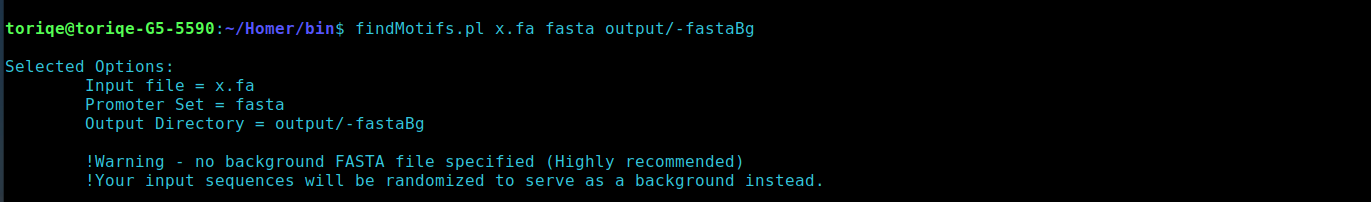
\includegraphics[width=0.5\columnwidth]{cmd.png} 
            \end{figure}
        \end{itemize}
        We didnot use any background fasta file.For details see \href{http://homer.ucsd.edu/homer/motif/fasta.html}{here}
\section{Results}
          \subsection{Experiment configuration}
          for each dataset we have run three different programs using 3 different techniques
          \textbf{Varied K from 8 to 24}
              \subsubsection{Program_1}
              \begin{itemize}
                  \item We selected N = 1000 and numberSeed = 50 for \href{https://github.com/Superb-Man/Bio-Info/blob/master/main.ipynb}{progarm1} 
                  \item We used Minimum hamming distance scoring technique for Randomized Motif Search and entropy technique for Giibs sampler which can be found in git repository from a \href{https://github.com/Superb-Man/Bio-Info/commit/92d92fe91373497ff0db6b44b64750403bce8eac}{commit} 
                  The Entropy Function is as follow :
                  \[
                    H(Nucleotide) = -\sum_{i=1}^{n} P(nuocleotide_i) \log_{2} P(nucleotide_i)
                    \]
                    
                    where $Nucleotide$ is a discrete random variable, $P(nucleotide_i)$ is the probability of the $i$-th outcome, and $n$ is the total number of possible outcomes. And
                    Nucleotide=['A','C','G','T']

              \end{itemize}
              \subsubsection{Progarm_2}
              \begin{itemize}
                  \item We selected N = 1000 and numberSeed = 50 for \href{https://github.com/Superb-Man/Bio-Info/blob/master/main_2.ipynb}{progarm2}
                  \item We used averege Information gain technique for finding motifs on both methods
                    \[
                    gain = \frac{maxEntropy*k - \sum_{i=1}^{k} H(Nucleotide)}{k}
                    \]
                where k denotes the motifs length
              \end{itemize}
            \subsubsection{Program3}
                \begin{itemize}
                    \item We selected N = 100 and numberSeed = 50 for \href{https://github.com/Superb-Man/Bio-Info/blob/master/main_3.ipynb}{progarm3} 
                    \item We tested with avg Minimum mismatch technique for both methods
                \end{itemize}
            \newpage
          \subsection{Comparison}
            \subsubsection{Progarm_3}
            \begin{figure}[htbp]
                \begin{minipage}[t]{0.5\columnwidth}
                    \centering
                    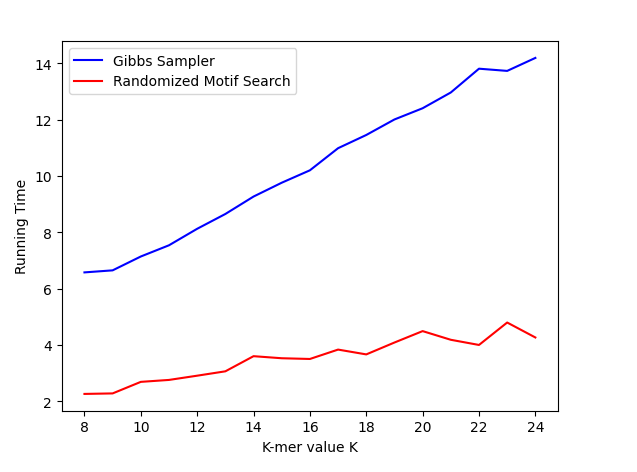
\includegraphics[width=0.5\columnwidth]{images/3-1.png} 
                    \caption{for \href{https://github.com/Superb-Man/Bio-Info/blob/master/data/hm03.txt}{dataset1}}
                    \label{fig:Fig-1}
                \end{minipage}
                \begin{minipage}[t]{0.5\columnwidth}
                    \centering
                    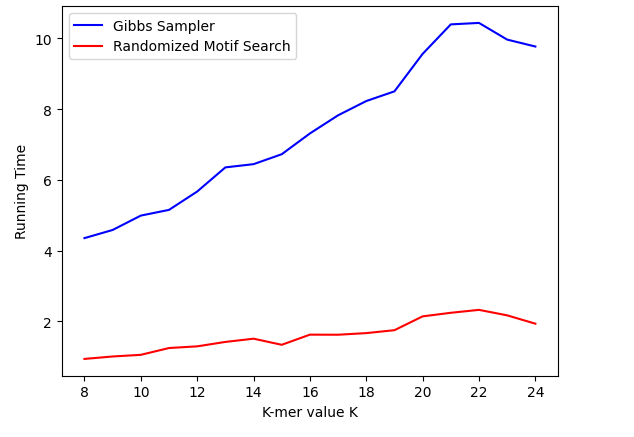
\includegraphics[width=0.5\columnwidth]{images/3-2.png} 
                    \caption{for \href{https://github.com/Superb-Man/Bio-Info/blob/master/data/yst04r.txt}{dataset2}}
                    \label{fig:Fig-2}
                \end{minipage}
                \begin{minipage}[t]{0.5\columnwidth}
                    \centering
                    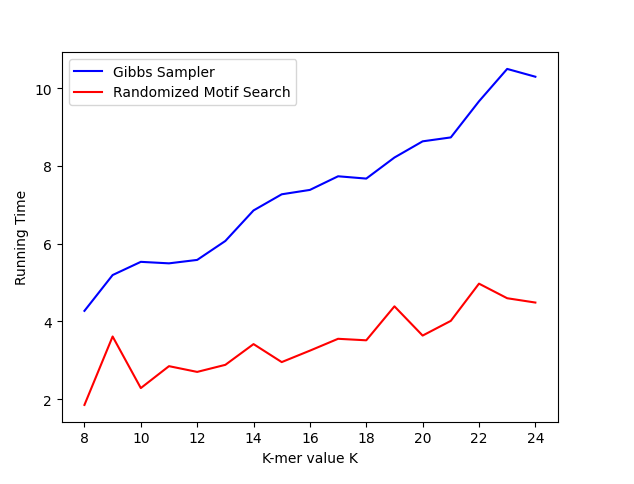
\includegraphics[width=0.5\columnwidth]{images/3-3.png} 
                    \caption{for \href{https://github.com/Superb-Man/Bio-Info/blob/master/data/yst08r.txt}{dataset3}}
                    \label{fig:Fig-3}
                \end{minipage}
                \begin{minipage}[t]{0.5\columnwidth}
                    \centering
                    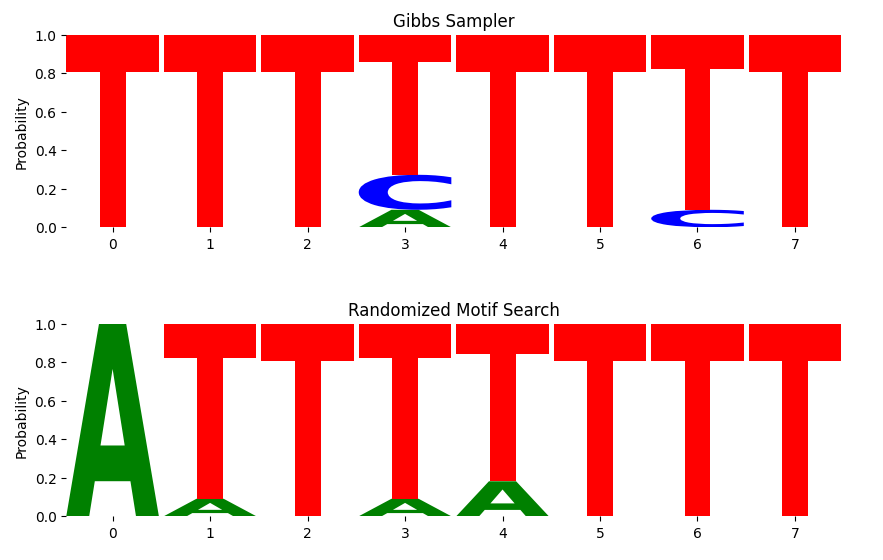
\includegraphics[width=0.5\columnwidth]{images/3-8.png} 
                    \caption{Best Motif Logo of K=8 \href{https://github.com/Superb-Man/Bio-Info/blob/master/data/yst08r.txt}{dataset3}}
                    \label{fig:Fig-4}
                \end{minipage}
            \end{figure}
            \begin{figure}[hbt!]
                \centering
                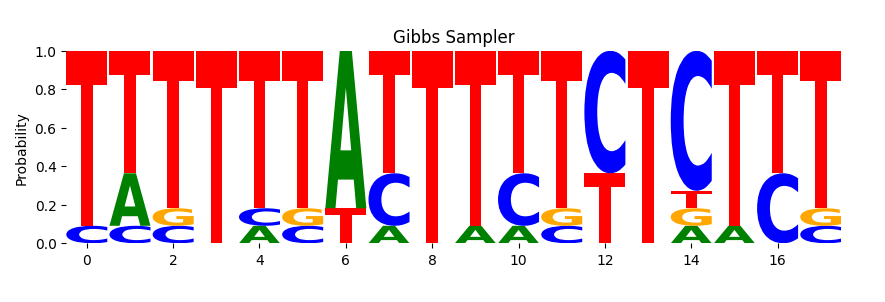
\includegraphics[width=0.5\columnwidth]{images/3-16.png} 
                \caption{Best Motif Logo of K=16 \href{https://github.com/Superb-Man/Bio-Info/blob/master/data/yst08r.txt}{dataset3}}
                \label{fig:Fig-5}
            \end{figure}
        \newpage
        \subsubsection{Progarm_2}
            \begin{figure}[htbp]
                \begin{minipage}[t]{0.5\columnwidth}
                    \centering
                    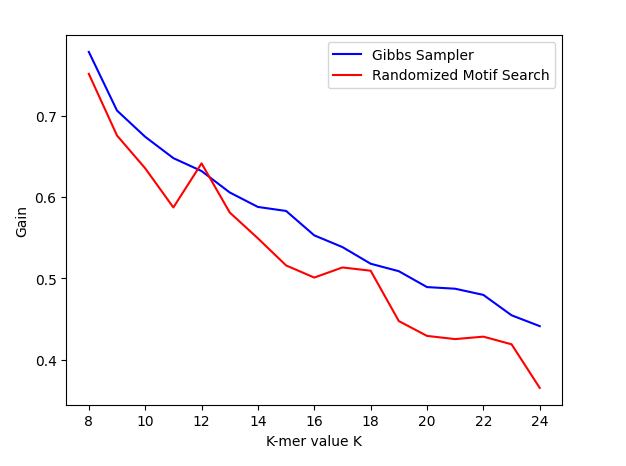
\includegraphics[width=0.5\columnwidth]{images/2-1.png} 
                    \caption{for \href{https://github.com/Superb-Man/Bio-Info/blob/master/data/hm03.txt}{dataset1}}
                    \label{fig:Fig-6}
                \end{minipage}
                \begin{minipage}[t]{0.5\columnwidth}
                    \centering
                    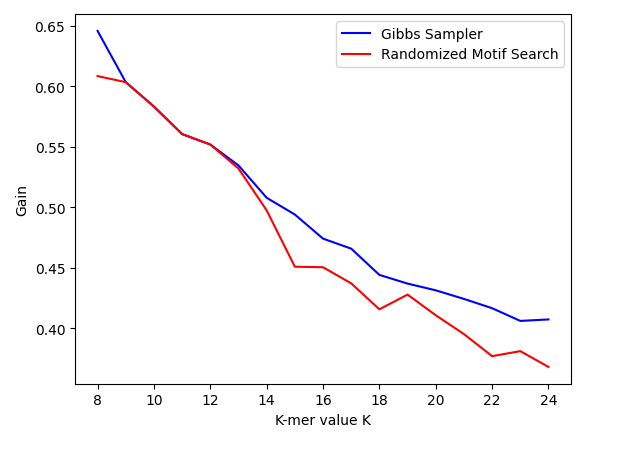
\includegraphics[width=0.5\columnwidth]{images/2-2.png} 
                    \caption{for \href{https://github.com/Superb-Man/Bio-Info/blob/master/data/yst04r.txt}{dataset2}}
                    \label{fig:Fig-7}
                \end{minipage}
                \begin{minipage}[t]{0.5\columnwidth}
                    \centering
                    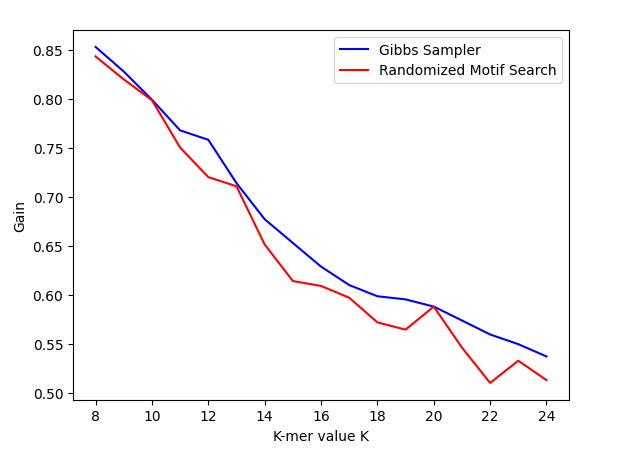
\includegraphics[width=0.5\columnwidth]{images/2-3.png} 
                    \caption{for \href{https://github.com/Superb-Man/Bio-Info/blob/master/data/yst08r.txt}{dataset3}}
                    \label{fig:Fig-8}
                \end{minipage}
                \begin{minipage}[t]{0.5\columnwidth}
                    \centering
                    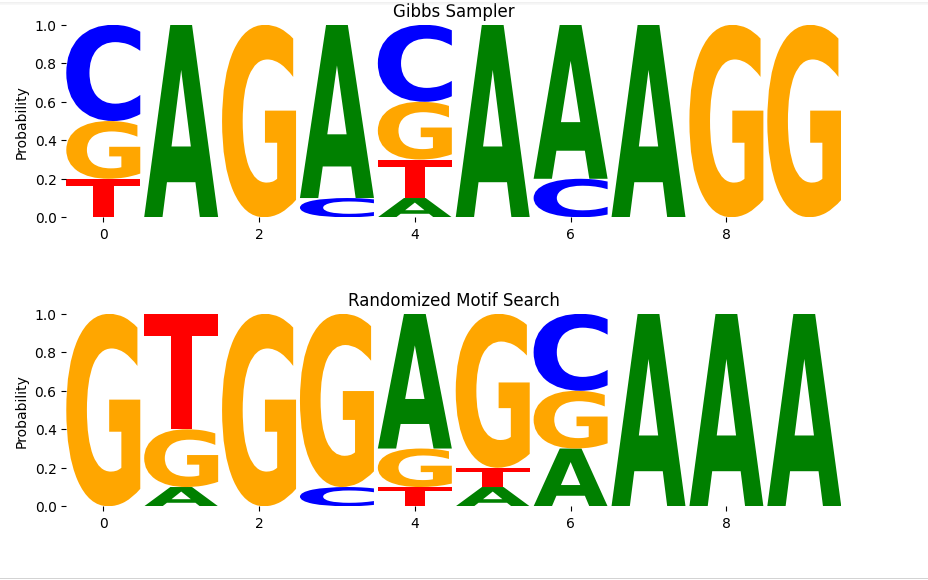
\includegraphics[width=0.5\columnwidth]{images/2-10.png} 
                    \caption{Best Motif Logo of K=10 \href{https://github.com/Superb-Man/Bio-Info/blob/master/data/hm03.txt}{dataset1}}
                    \label{fig:Fig-9}
                \end{minipage}
            \end{figure}

        \subsubsection{Homer and RSAT Output for Dataset1}
            \begin{figure}[hbt!]
                \centering
                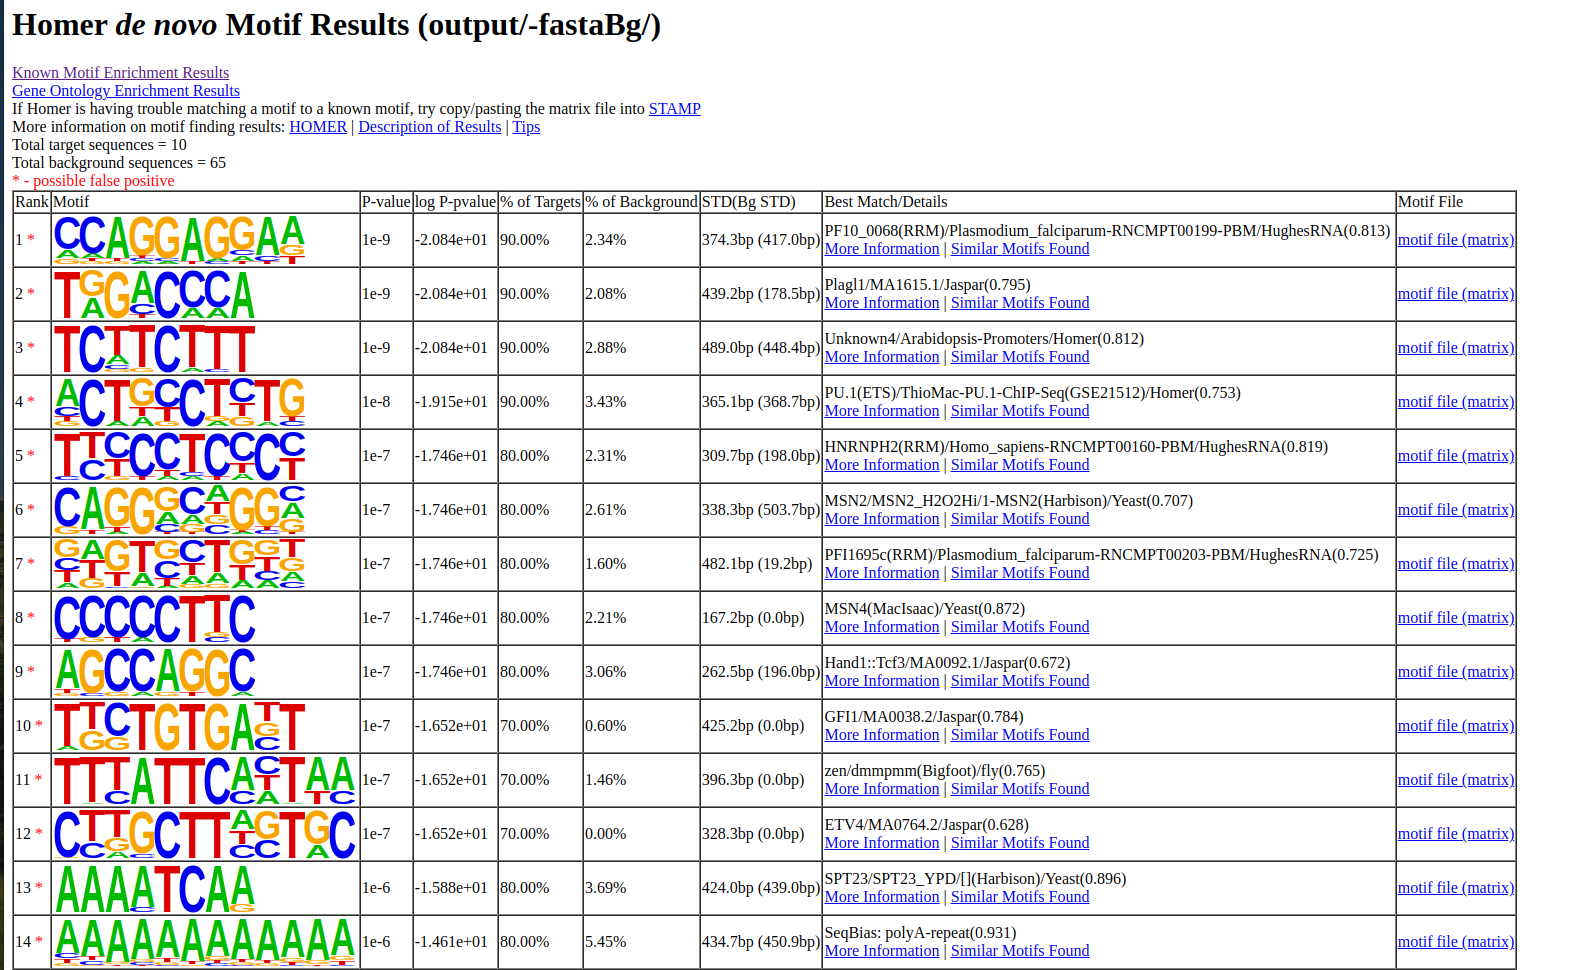
\includegraphics[width=0.5\columnwidth]{images/Homer.png} 
                \caption{\href{https://github.com/Superb-Man/Bio-Info/blob/master/output/-fastaBg/homerResults.html}{Homer Result for hm03 dataset}}
                \label{fig:Fig-10}
            \end{figure}
             \begin{figure}[hbt!]
                \centering
                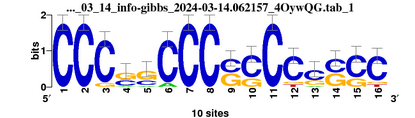
\includegraphics[width=0.5\columnwidth]{images/RSAT.png} 
                \caption{RSAT Result for hm03 dataset, K=16,numSeed=10,iteration=1000}
                \label{fig:Fig-11}
            \end{figure}
        
        
        
          
          
\section{Conclusion}
We see from Figure\ref{fig:Fig-1}, Figure\ref{fig:Fig-2}, Figure\ref{fig:Fig-3} \textbf{Randomized Motif Search} works significantly faster than \textbf{Gibbs Sampling}. When we vary the value of K and tends to increase it ,the running time for Gibbs sampler increases. But we can see from Figure\ref{fig:Fig-6}, Figure\ref{fig:Fig-7} and Figure\ref{fig:Fig-8} that Gibbs sampler gives much more statistically significant output as the Information-gain is larger and entropy is lower for Gibbs Sampler method.From those plots we also observe that for larger K the gain difference begins to increase than it was before.In the Homer tool testing the results of different K's are ranked.This is because they used some sophisticated scoring technique using mean,deviation,expected values [\href{http://homer.ucsd.edu/homer/motif/index.html}{here}] and they used a background fasta file for finding motifs which results statistically more accurate.We tested the RSAT tool output entropy and it was a little bit larger than our implementation result.
Homer and RSAT both uses Gibbs Sampler by default.
\section{References}
\begin{itemize}
    \item \href{https://academic.oup.com/nar/article/50/W1/W670/6584431}{RSAT Article}
    \item \href{http://rsat.sb-roscoff.fr/info-gibbs_form.cgi}{RSAT GibbsSampler}
    \item \href{http://homer.ucsd.edu/homer/motif/}{Homer Motifs}
    \item \href{https://www.ncbi.nlm.nih.gov/pmc/articles/PMC4763482/}{Homer Article}
    \item  \href{https://github.com/Superb-Man/Bio-Info/tree/master/data}{Datasets}
\end{itemize}
\end{document}
